\section{Synchronmaschine}
\s{Die Synchronmaschine ist eine Drehfeldmaschine, die folglich mit einem dreiphasigen Drehstrom (siehe Modul 7) im Statorkreis betrieben wird. Der Rotor kann entweder permanent (mit Dauermagneten) oder durch einen Gleichstromkreis erregt werden. Dieser Maschinentyp wird in Kraftwerken zur Stromgewinnung eingesetzt, da er aber über einen sehr hohen Wirkungsgrad verfügt, wird er auch in der modernen Antriebstechnik in kleineren Leistungsklassen immer häufiger eingesetzt. Ein wesentlicher Nachteil besteht jedoch darin, dass die Synchronmaschine immer durch eine Leistungselektronik geregelt werden muss, da sie an einem einfachen Drehstromnetz nicht anläuft.}
\vspace{0.5cm}

\begin{frame}
	\ftx{Synchronmaschine}
	\b{Die Synchronmaschine dreht netzsynchron mit konstanter Drehzahl}
	\textbf{Vorteile:}
	\begin{itemize}
		\item Robust und wartungsfrei.
		\item Hohe Regeldynamik.
		\item Hohe Leistungsdichte bei geringem Bauvolumen.
		\item Überlastfähigkeit.
	\end{itemize}\pause
	\textbf{Nachteile:}
	\begin{itemize}
		\item Aufwendige Umrichtertechnik.
		\item Aufwendige Regelung.
		\item Gesteuerter Betrieb nur mit großem Aufwand oder gar nicht möglich.
	\end{itemize}
\end{frame}

\s{\subsection{Aufbau}\index{Synchronmaschine>Aufbau}}
\begin{frame}
	\ftx{Aufbau einer fremderregten Synchronmaschine}
	\begin{columns}
		\column[c]{0.55\textwidth}
		\begin{itemize}
			\item Drei Statorwicklungen, die 120° zueinander versetzt sind.
			\item Geblechte Ausführung des Stators, da dieser ein magnetisches Wechselfeld erfährt.
			\item Im Läufer befindet sich die Erregerwicklung.
			\item Der Läufer wird teilweise nicht geblecht.
		\end{itemize}
		\column[c]{0.45\textwidth}
		\s{
			\fo{width=0.7\textwidth}{}{Aufbau_Synchronmaschine1}{
				\put(83,0){\line(-1,1){37.5}}\put(83.3,0){Statorwicklungen}
				\put(83,6){\line(-1,1){33.5}}\put(83.3,6){Statorblechpaket}
				\put(89,18){\line(-1,1){32}}\put(89.3,18){Erregerwicklung}
				\put(89,24){\line(-1,1){35}}\put(89.3,24){Läufer}
				\put(100,36){\line(-1,1){26.2}}\put(100.3,36){Lager}
				\put(100,42){\line(-1,1){26.2}}\put(100.3,42){Gehäuse}
			}{{\bf Grafik einer aufgeschnittenen fremderregten Synchronmaschine.}}
			\vspace{0.5cm}
		}
		\b{
			\f{}{width=\textwidth}{Aufbau_Synchronmaschine1}{}
		}
	\end{columns}
\end{frame}

\begin{frame} \ftx{Aufbau einer fremderregten Synchronmaschine}
	\s{
		\fo{width=0.8\textwidth}{}{Aufbau_Synchronmaschine2}{
			\put(32.3,16.1){\line(1,1){15}}\put(11,16.1){Statorwicklung 1}
			\put(86,66){\line(-1,-1){12.7}}\put(86.3,66){Statorwicklung 2}
			\put(91,10.4){\line(-1,1){12.4}}\put(91.3,10.4){Statorwicklung 3}
		}{{\bf Aufbau einer fremderregten Synchronmaschine.} Die um 120° zueinander versetzten Statorwicklungen sind hier farbig veranschaulicht.}
	}
	\b{
		\foo{}{width=0.75\textwidth}{Aufbau_Synchronmaschine2}{
			\put(32.3,16.1){\line(1,1){15}}\put(6.3,16.1){Statorwicklung 1}
			\put(86,66){\line(-1,-1){12.7}}\put(86.3,66){Statorwicklung 2}
			\put(91,10.4){\line(-1,1){12.4}}\put(91.3,10.4){Statorwicklung 3}
		}{}
	}
	
\end{frame}



\begin{frame}\ftb{Feldverläufe}
	\s{
		\fo{width=\textwidth}{}{Synchronmaschine_Feldverlaeufe}{
			\put(10.23,23.3){{\begin{tikzpicture}[domain=0:36, samples=360, scale=0.982]
	\foreach \n in {0,...,3}{
		\draw[very thin, color=gray] (\n*4, 1) -- (\n*4,-1.5);
	}
	\draw (-0.1,0) -- (12.1,0);
	\draw[->] (0,-1.1) -- (0,1.2) node[above] {$I$};
	\draw (0.1, 0) node[below] {0};
	\foreach \n in {1,...,6}{
		\draw (\n*2, 0.1) -- (\n*2,-0.1);
		\fill[fill=white] (\n*2 - 0.1,-0.5) rectangle ++(0.2,0.4); % weißes Overlay über Linie hinter Zahlen
		\draw (\n*2, 0) node[below] {\pgfmathparse{60*\n}\pgfmathprintnumber[]{\pgfmathresult}\degree};
	}
	\draw[color=statorw1, scale=1/3, smooth, very thick] plot[id=drehfeldverlauf1] function{3 * cos(0.0556 * pi * x)};
	\draw[color=statorw1] (1.8,0.55) node[above] {$I_1$};
	\draw[color=statorw2, scale=1/3, smooth, very thick] plot[id=drehfeldverlauf3] function{3 * cos(0.0556 * pi * x - pi * 2/3)};
	\draw[color=statorw2] (5.8,0.55) node[above] {$I_2$};
	\draw[color=statorw3, scale=1/3, smooth, very thick] plot[id=drehfeldverlauf2] function{3 * cos(0.0556 * pi * x + pi * 2/3)};
	\draw[color=statorw3] (9.8,0.55) node[above] {$I_3$};
	\end{tikzpicture}
}
			}
			
			\put(12.5, 21.5){\color{statorw1}$I_1$} \put(38, 21.5){\color{statorw1}$I_1$} \put(63.6, 21.5){\color{statorw1}$I_1$} \put(89.3, 21.5){\color{statorw1}$I_1$}
			\put(21, 1.5){\color{statorw2}$I_2$} \put(47, 1.5){\color{statorw2}$I_2$} \put(73, 1.5){\color{statorw2}$I_2$} \put(98, 1.5){\color{statorw2}$I_2$}
			\put(0, 1.5){\color{statorw3}$I_3$} \put(25.5, 1.5){\color{statorw3}$I_3$} \put(51, 1.5){\color{statorw3}$I_3$} \put(77, 1.5){\color{statorw3}$I_3$}
		}{{\bf Richtung des Drehfeldvektors.} Der Rotor dreht sich synchron zu den sinusförmigen, um 120$\degree$ zueinander versetzten Drehfeldern des Stators.}
	}
	\b{
		\foo{}{height=0.8\textheight}{Synchronmaschine_Feldverlaeufe_a1}{
			\put(-47,60){\begin{tikzpicture}[domain=0:0.3, samples=360, scale=0.838]
					\foreach \n in {1,...,4}{
							\draw[very thin, color=gray] (\n*4, 1) -- (\n*4,-1);
						}
					\draw (-0.1,0) -- (12.1,0);
					\draw[->] (0,-1.1) -- (0,1.2) node[above] {$I$};
					\draw (0.2, 0) node[below] {0};
					\foreach \n in {1,...,6}{
							\draw (\n*2, 0.1) -- (\n*2,-0.1);
							\fill[fill=white] (\n*2 - 0.1,-0.6) rectangle ++(0.2,0.5); % weißes Overlay über Linie hinter Zahlen
							\draw (\n*2, 0) node[below] {\pgfmathparse{60*\n}\pgfmathprintnumber[]{\pgfmathresult}\degree};
						}
					\draw[color=statorw1, scale=1/3, smooth, very thick] plot[id=drehfeldverlauf1a1] function{3 * cos(0.0556 * pi * x)};
					\draw[color=statorw1] (-0.3,0.55) node[above] {$I_1$};
					\draw[color=statorw2, scale=1/3, smooth, very thick] plot[id=drehfeldverlauf3a1] function{3 * cos(0.0556 * pi * x - pi * 2/3)};
					\draw[color=statorw2] (-0.3,-0.1) node[above] {$I_2$};
					\draw[color=statorw3, scale=1/3, smooth, very thick] plot[id=drehfeldverlauf2a1] function{3 * cos(0.0556 * pi * x + pi * 2/3)};
					\draw[color=statorw3] (-0.3,-0.75) node[above] {$I_3$};
				\end{tikzpicture}
			}
			\put(28, 51){\color{statorw1}$I_1$}
			\put(48, 3){\color{statorw2}$I_2$}
			\put(-1, 3){\color{statorw3}$I_3$}
		}{}
	}
\end{frame}

\b{ % Quasi-Animation für Vorlesungsdatei
	\begin{frame}\ftb{Feldverläufe}
		\foo{}{height=0.8\textheight}{Synchronmaschine_Feldverlaeufe_a2}{
			\put(-47,60){\begin{tikzpicture}[domain=0:12, samples=360, scale=0.838]
					\foreach \n in {1,...,4}{
							\draw[very thin, color=gray] (\n*4, 1) -- (\n*4,-1);
						}
					\draw (-0.1,0) -- (12.1,0);
					\draw[->] (0,-1.1) -- (0,1.2) node[above] {$I$};
					\draw (0.2, 0) node[below] {0};
					\foreach \n in {1,...,6}{
							\draw (\n*2, 0.1) -- (\n*2,-0.1);
							\fill[fill=white] (\n*2 - 0.1,-0.6) rectangle ++(0.2,0.5); % weißes Overlay über Linie hinter Zahlen
							\draw (\n*2, 0) node[below] {\pgfmathparse{60*\n}\pgfmathprintnumber[]{\pgfmathresult}\degree};
						}
					\draw[color=statorw1, scale=1/3, smooth, very thick] plot[id=drehfeldverlauf1a2] function{3 * cos(0.0556 * pi * x)};
					\draw[color=statorw1] (-0.3,0.55) node[above] {$I_1$};
					\draw[color=statorw2, scale=1/3, smooth, very thick] plot[id=drehfeldverlauf3a2] function{3 * cos(0.0556 * pi * x - pi * 2/3)};
					\draw[color=statorw2] (-0.3,-0.1) node[above] {$I_2$};
					\draw[color=statorw3, scale=1/3, smooth, very thick] plot[id=drehfeldverlauf2a2] function{3 * cos(0.0556 * pi * x + pi * 2/3)};
					\draw[color=statorw3] (-0.3,-0.75) node[above] {$I_3$};
				\end{tikzpicture}
			}
			\put(28, 51){\color{statorw1}$I_1$}
			\put(48, 3){\color{statorw2}$I_2$}
			\put(-1, 3){\color{statorw3}$I_3$}
		}{}
	\end{frame}
	\begin{frame}\ftb{Feldverläufe}
		\foo{}{height=0.8\textheight}{Synchronmaschine_Feldverlaeufe_a3}{
			\put(-47,60){\begin{tikzpicture}[domain=0:24, samples=360, scale=0.838]
					\foreach \n in {1,...,4}{
							\draw[very thin, color=gray] (\n*4, 1) -- (\n*4,-1);
						}
					\draw (-0.1,0) -- (12.1,0);
					\draw[->] (0,-1.1) -- (0,1.2) node[above] {$I$};
					\draw (0.2, 0) node[below] {0};
					\foreach \n in {1,...,6}{
							\draw (\n*2, 0.1) -- (\n*2,-0.1);
							\fill[fill=white] (\n*2 - 0.1,-0.6) rectangle ++(0.2,0.5); % weißes Overlay über Linie hinter Zahlen
							\draw (\n*2, 0) node[below] {\pgfmathparse{60*\n}\pgfmathprintnumber[]{\pgfmathresult}\degree};
						}
					\draw[color=statorw1, scale=1/3, smooth, very thick] plot[id=drehfeldverlauf1a3] function{3 * cos(0.0556 * pi * x)};
					\draw[color=statorw1] (-0.3,0.55) node[above] {$I_1$};
					\draw[color=statorw2, scale=1/3, smooth, very thick] plot[id=drehfeldverlauf3a3] function{3 * cos(0.0556 * pi * x - pi * 2/3)};
					\draw[color=statorw2] (-0.3,-0.1) node[above] {$I_2$};
					\draw[color=statorw3, scale=1/3, smooth, very thick] plot[id=drehfeldverlauf2a3] function{3 * cos(0.0556 * pi * x + pi * 2/3)};
					\draw[color=statorw3] (-0.3,-0.75) node[above] {$I_3$};
				\end{tikzpicture}
			}
			\put(28, 51){\color{statorw1}$I_1$}
			\put(48, 3){\color{statorw2}$I_2$}
			\put(-1, 3){\color{statorw3}$I_3$}
		}{}
	\end{frame}
	\begin{frame}\ftb{Feldverläufe}
		\foo{}{height=0.8\textheight}{Synchronmaschine_Feldverlaeufe_a1}{
			\put(-47,60){\begin{tikzpicture}[domain=0:36, samples=360, scale=0.838]
					\foreach \n in {1,...,4}{
							\draw[very thin, color=gray] (\n*4, 1) -- (\n*4,-1);
						}
					\draw (-0.1,0) -- (12.1,0);
					\draw[->] (0,-1.1) -- (0,1.2) node[above] {$I$};
					\draw (0.2, 0) node[below] {0};
					\foreach \n in {1,...,6}{
							\draw (\n*2, 0.1) -- (\n*2,-0.1);
							\fill[fill=white] (\n*2 - 0.1,-0.6) rectangle ++(0.2,0.5); % weißes Overlay über Linie hinter Zahlen
							\draw (\n*2, 0) node[below] {\pgfmathparse{60*\n}\pgfmathprintnumber[]{\pgfmathresult}\degree};
						}
					\draw[color=statorw1, scale=1/3, smooth, very thick] plot[id=drehfeldverlauf1] function{3 * cos(0.0556 * pi * x)};
					\draw[color=statorw1] (-0.3,0.55) node[above] {$I_1$};
					\draw[color=statorw2, scale=1/3, smooth, very thick] plot[id=drehfeldverlauf3] function{3 * cos(0.0556 * pi * x - pi * 2/3)};
					\draw[color=statorw2] (-0.3,-0.1) node[above] {$I_2$};
					\draw[color=statorw3, scale=1/3, smooth, very thick] plot[id=drehfeldverlauf2] function{3 * cos(0.0556 * pi * x + pi * 2/3)};
					\draw[color=statorw3] (-0.3,-0.75) node[above] {$I_3$};
				\end{tikzpicture}
			}
			\put(28, 51){\color{statorw1}$I_1$}
			\put(48, 3){\color{statorw2}$I_2$}
			\put(-1, 3){\color{statorw3}$I_3$}
		}{}
	\end{frame}
}


\begin{frame}\ftx{Feldverläufe}
	\s{Bei der Synchronmaschine bewirkt die magnetische Kopplung zwischen Stator und Rotor das Drehmoment. Im Motorbetrieb folgt das Rotorfeld dem Statorfeld. Die mechanische Drehzahl muss daher immer gleich der elektrischen Drehfrequenz sein. Zwischen dem Stator und dem Rotor befindet sich der lastabhängige sogenannte Polradwinkel\index{Polradwinkel} $\vartheta$. \nomenclature[F]{$\vartheta$}{Polradwinkel der Synchronmaschine \nomunit{$\degree$}} Bei $\vartheta=90\degree$ ist das Drehmoment am größten. Wird im Motorbetrieb der Polradwinkel durch eine zu hohe Belastung größer als $90\degree$, sinkt das erzeugte Drehmoment und die Maschine \glqq kippt\grqq -- das heißt, sie bleibt schlagartig stehen.}
	\begin{itemize}
		\item Der Statorfluss entsteht durch die Überlagerung der Flüsse der drei Wicklungen.
		      \uncover<2>{\item Der Läuferfluss entsteht durch die Erregerwicklung.}
	\end{itemize}
	
\end{frame}

\begin{frame}\ftx{Drehmoment}
	\fu{
		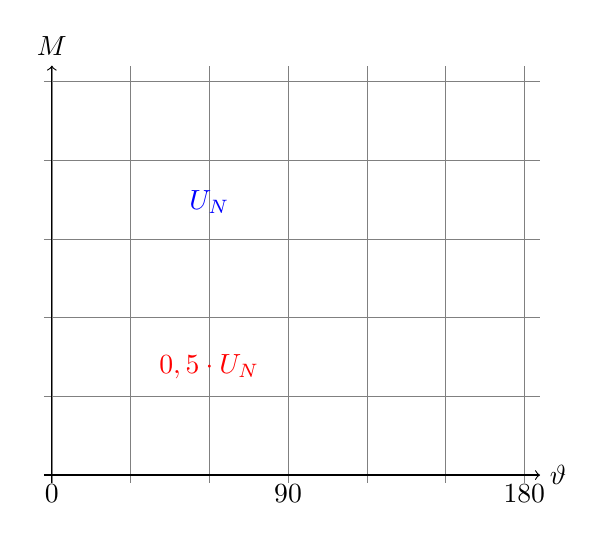
\begin{tikzpicture}[domain=0:6, samples=200]
	\draw[very thin,color=gray] (-0.1,-0.1) grid (6.2,5.2);
	\draw[->] (-0.1,0) -- (6.2,0) node[right] {$\vartheta$};
	\draw[->] (0,-0.1) -- (0,5.2) node[above] {$M$};
	\draw[color=red, smooth] plot[id=drehmomentkennlinie1] function{-x*x / 4 + 1.5 * x};
	\draw[color=red] (2,1.1) node[above] {$0,5\cdot U_N$};
	\draw[color=blue, smooth] plot[id=drehmomentkennlinie2] function{-x*x / 2 + 3 * x };
	\draw[color=blue] (2,3.2) node[above] {$U_N$};
	\draw (0,0) node[below] {0\degree};
	\draw (3,0) node[below] {90\degree};
	\draw (6,0) node[below] {180\degree};
\end{tikzpicture}
	}{{\bf Drehmomentkennlinie in Abhängigkeit vom Polradwinkel.}}
\end{frame}


\s{\subsection{Ersatzschaltbild \index{Synchronmaschine>Ersatzschaltbild}}}
\begin{frame}
	\ftx{Einphasiges ESB}
	\s{Im Netzbetrieb ist die Klemmenspannung $U_1$ und die Frequenz $\omega$ fest vorgegeben. Das ist ein häufiger Betriebsfall für die Synchronmaschine.}
	\b{Komplexes einphasiges ESB des Vollpolgenerators (z.B. im Netzbetrieb):}
	\fu{
		\begin{circuitikz}[scale=0.75]
	\draw (0,4)
	to[short,o-,i=$\underline{I}_1$](1,4)
	to[R, l=$R_1$](3,4)
	to[L, l=$X_{1\sigma}$, -*](5,4)
	to[L, l=$X_\mathrm{h}$](7,4)
	to[V, v=$\underline{U}_\mathrm{p}$](7,0)
	to[short,-*] (5,0)
	to[short,-o] (0,0);
	\draw (0,0) to[open, l=$\underline{U}_1$] (0,4)
	(0,0.5) [->] (0,3.5) -- (0,0.5);
	\draw (5,0) to[open, l=$\underline{U}_\mathrm{q}$] (5,4)
	(5,0.5) [->] (5,3.5) -- (5,0.5);
	\draw (9,1)
	to[short, o-](9,2)
	to[L](11,2)
	to[short, -o, i=$I_\mathrm{E}$](11,1);
\end{circuitikz}
		}{{\bf Komplexes einphasiges ESB eines Vollpolgenerators.} Beispielsweise im Netzbetrieb.}
\end{frame}





